\documentclass[conference]{IEEEtran}
\IEEEoverridecommandlockouts
% The preceding line is only needed to identify funding in the first footnote. If that is unneeded, please comment it out.
\usepackage{cite}
\usepackage{amsmath,amssymb,amsfonts}
\usepackage{algorithmic}
\usepackage{graphicx}
\usepackage{textcomp}
\usepackage{xcolor}
\def\BibTeX{{\rm B\kern-.05em{\sc i\kern-.025em b}\kern-.08em
    T\kern-.1667em\lower.7ex\hbox{E}\kern-.125emX}}
\begin{document}

\title{Game Theory. \\ Practical Assignment 2. Report.}

\author{\IEEEauthorblockN{Artem Chernitsa}
\IEEEauthorblockA{\textit{student, group BAI-01} \\
\textit{Innopolis University}\\
Innopolis, Russia \\
a.chernitsa@innopolis.university}
}

\maketitle

\begin{abstract}
This document is a report for the practical assignment on Game Theory course Fall 2022. It includes problem description, theoretical computations, description of proposed solution, important parts of implementation.
\end{abstract}

\begin{IEEEkeywords}
game theory, non-zero-sum games, axelrod's tournament, the prisoner's dilemma, snowball game
\end{IEEEkeywords}

\section{Introduction}
Snowball game is an example of a non-zero-sum game, and axelrod's tournament, which, for understanding, requires a description to understand the nature of this game. In short, two players play against each other on a large field divided into three parts: one for each player and one common zone. Players throw snowballs either onto each other's field, or into a common area where snowballs disappear forever within the game. Every minute a snowball is added to the field with the help of a Snowball Generator Machine (SGM). The goal of each player is to minimize the number of snowballs in their half after 60 minutes. The most important thing is that the players play in the tournament, each with each once, and the rating of each player depends on the total number of remaining snowballs on his half for all the matches played.

\section{Problem Description}

% \subsection{Maintaining the Integrity of the Specifications}

The environment where players play the snowball game is three territorial regions which we will helpfully entitled as A, B, and C fields. Fields A and B contain one player on each side. The field C does not contain any players and should be considered as a hot field where snowballs automatically melt and disappear. The players cannot change their positions and should shot snowballs from the field they are located on. 

Let assume that for both A and B fields the initial number of snowballs is $N=100$. Each A and B fields have a single SGM. Because of those machines each imaginary minute the number of snowballs $N$ increases by 1 for both fields.

Both players are using special Snowball Cannons (SC) able to shoot snowballs. Assume that shooting does not melt or destroy snowballs. The players can use Cannons at most once per minute to opponent’s field and at most once per minute to hot field (totally at most twice, assume it as sequential shots, where shot to opponent’s field happens firstly). Each shot can contain 1 snowball or more. Not shooting is also allowed and requires 0 to be returned by a proper method. If no shooting happened to opponent’s and hot fields, then it is assumed that during this minute shooting did not happen. If SC was used once or twice per minute, then it is assumed as a presence of shooting during this minute. However, the shooting history affects the maximum number of snowballs shoot for the next minutes. The maximum number of snowballs shoot by cannon per minute (together for both shots) is defined by equation
\begin{equation}
f(x) = \left \lfloor \cfrac{15 \cdot e^x}{15 + e^x} \right \rfloor\label{eq1}
\end{equation}

\section{Theoretical Computations}
\subsection{Calculating Rates}
Since we will have to adjust the strategy depending on the opponent's behavior according to \cite{b2}, it is necessary to get the maximum available information. To this end, we will first calculate the maximum possible number of snowballs at each waiting interval.

\begin{figure}[htbp]
\centerline{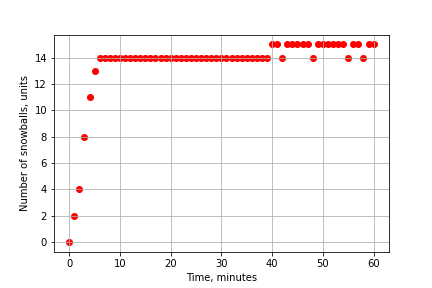
\includegraphics[width=0.5\textwidth]{fig1_maximum_snowball_per_round.png}}
\caption{Dependency the maximum number of snowballs on time t.}
\label{fig}
\end{figure}

As shown in Fig.1 the maximum possible number of balls to throw is 15. However, this amount is reached only after 40 minutes of waiting. Without taking into account SGM, we will be able to throw only 15 balls out of 100. the calculated maximum speeds of throwing snowballs per minute show that the fastest way to throw snowballs is 11 units every 4 minutes. Thus, the speed will be 2.75 snowballs / minute (s/m). For comparison, in Tab.1 all calculated rates are presented.

\begin{table}[htbp]
\caption{Maximum Possible Snowball Rates}
\begin{center}
\begin{tabular}{|c|c|c|}
\hline
\textbf{Snowballs}&\textbf{Interval}&\textbf{Rate, $s/m$} \\
\hline
15& 40& 0.375 \\
\hline
14& 6& 2.3 \\
\hline
13& 5& 2.6 \\ 
\hline
11& 4& 2.75 \\
\hline
8& 3& 2.66 \\
\hline
4& 2& 2.0 \\
\hline
2& 1& 2.0 \\
\hline
\end{tabular}
\label{tab1}
\end{center}
\end{table}


% Before you begin to format your paper, first write and save the content as a 
% separate text file. Complete all content and organizational editing before 
% formatting. Please note sections \ref{AA}--\ref{SCM} below for more information on 
% proofreading, spelling and grammar.

% Keep your text and graphic files separate until after the text has been 
% formatted and styled. Do not number text heads---{\LaTeX} will do that 
% for you.

\subsection{Analysis of Opponent Data}
After each round (or time), information is available about how many snowballs flew to our half from the opponent's side. We can assume the upper limit of the number of opponent's snowballs, but it will not be possible to know for sure the exact number, because we do not have information about how many balls the opponent decided to throw in general and how many of them he threw into the "neutral" zone.

Assume that the opponent is trying to maximize each step, then if $n_t$ number of snowballs in time $t$ arrived on our half, therefore the opponent has a maximum of $S_{t+1} - n_t$ snowballs, where $S_{t+1}$ is the estimated number of snowballs of the opponent on time $t+1$. It also turns out that the opponent will throw a total of 11 snowballs every 4 minutes, because this is the fastest way to get rid of the snowballs. Let's also take into account SGM emissions, which add one snowball to each side every minute.

So, every four minutes we have a chance to get maximum 15 snowballs in total (11 from opponent and 4 from SGM). This means that in the last round we may have 14 * 11 + 60 + 3 * 2 = 220 snowballs, in addition to the ones we already had at the beginning of the game.

\section{Strategy Choosing}

As we assumed before, opponent plays optimal, therefore the optimal strategy for both players is to "burn" snowballs, throwing it to the "neutral" zone. In that sense we simply "burn" snowballs with maximum rate. However, we could not be sure, that opponent will play optimal in this sense. Then we three choices:
\begin{enumerate}
\item Continue "burn" snowballs.
\item Throw back $k$ number of snowballs and "burn" the rest with the maximum rate.
\item Respond to a "bad" action by the number of mistakes of the opponent.
\end{enumerate}

\subsection{Continue "Burn" Snowballs}
With optimal play on both sides, players can completely get rid of snowballs on each of the halves, because in 57 minutes each of them can throw 154 snowballs to "burn", and in another 3 minutes they can throw the remaining 6 snowballs.

\subsection{Throw back $k$ number of snowballs and "burn" the rest with the maximum rate}
It may seem that a possible solution to the problem would be to throw some snowballs at the enemy, and burn some. However, such behavior will not be beneficial if the enemy responds to us. Firstly, we will lower the speed of burning snowballs, and secondly, we will not keep up with the enemy in an effective way. If we want to answer the enemy that we will have to throw all 11 snowballs every 4 minutes, but then we will not burn them. In the end, this approach turns into either approach number 1 or the opposite, when we throw all the snowballs at the enemy.

\subsection{Respond to a "bad" action by the number of mistakes of the opponent}
Throw snowballs in response to each throw of the opponent in half of the player. Moreover, it is important to make two return throws whenever possible in order to restore the previous value of the balls and get rid of the extra ones. Unfortunately, it can be taken into account that it does not make sense for the opponent to play randomly and, i.e., it can be assumed that all his actions are strictly deterministic, then when throwing on the player's field, it can be assumed that the throws will continue, so we will try to minimize losses in the case of a throw in our direction. If the throws are not constant, then we respond so as to get rid of extra snowballs. It is worth noting that with mutual transfers, the minute at which this happened for the first time fixes the number of snowballs for both players and this number will only increase by the end of the match due to SGM.

The answer option allows you to minimize losses with a difference of one move. If it turned out that the opponent threw snowballs to the player's side first, then the player will have a backlog of 11 balls. Moreover, if the opponent started with a favorable throw, but the player did not, then the gap may be greater, up to 14 snowballs at the end of the match. 

\section{Observations}
\subsection{Critical number of players}
Firstly, I would like to note that throwing snowballs or burning them is beneficial starting with waiting three minutes for the first throw so that at the last minute you can throw 11 snowballs, instead of the maximum possible 8. Secondly, the policy of cooperation, which is called the "optimal" strategy has a significant drawback, it assumes a significant number of students will play "optimally". For example, if 9 out of 10 players play aggressively (throwing from the first effective minute of the player), then the player will have the most snowballs at the end of the tournament. It is necessary to solve the inequality (Eq. 2) in order to estimate the upper limit of the number of "aggressive" players in order to guarantee the minimum total number of snowballs at the end of the tournament. Consider the equation for a specific player:

\begin{equation}
\begin{split}
(n - k - 1) \cdot (11 + b) < (n - k - 1) \cdot b + k \cdot (b - 11)
% 11k + kb - 11 - b < 2nb - 2bk - 2b\\
% k(11 + 3b) - 11 + b(1 - 2n) < 0
\end{split}
\end{equation}

Where $n$ - total number of participants, $k$ - number of "optimal" players, $b$ - accumulated losses (in our case simply number of snowballs at the beginning of the game plus the machine generated for the entire match).

The minimum threshold of "optimal" players for $n = 60$ was calculated, which was 6 people. That is, if at least 6 people play "optimally", then this guarantees the minimum number of points. This is another reason for choosing the "optimal" strategy over the "aggressive" one.

\subsection{Naive agent beats "optimal" one}
When modeling the tournament, the unaccounted behavior of a naive player (who always throws snowballs into the hot zone) was noticed. It is interesting that if in a tournament, when recruiting only from "optimal" and naive players, the first ones will always win as opposed to a strategy where we don't throw snowballs at the opponent on the last move \cite{b1, b3}. But as soon as "aggressive" players are added to them, naive ones collect the minimum number of points at the end of the tournament at the expense of "optimal" ones. This happens because when playing "aggressive" and "optimal", the latter experiences losses of 8 points, and when playing with a naive one, it beats these 8 points back, i.e. it simply maintains balance. However, when the "aggressive" plays with the naive, the latter can throw 11 snowballs in the last round, instead of 8, which is 3 more. Thus, as soon as 2 "optimal" agents appear, and the number of "aggressive" ones exceeds or equals three, the naive ones break out due to their interaction with each other.

\section{Conclusion}
This means that we can more likely guarantee the second resulting place in the tournament for the "optimal" strategy, assuming that the number of each type of player will not fall below the critical minimum, which is quite justified for about 60 people. In addition, we cannot memorize the game with other agents according to the rules, which means we cannot understand for sure which of the three strategies we should adopt in the current situation.

Taking into account the above, it was decided to choose the "optimal" strategy for the agent, because it minimizes the risk of losses, and can more likely than other strategies to guarantee a place in the tournament not lower than the second result.


\begin{thebibliography}{00}
\bibitem{b1} R. M. Axelrod, The Evolution of Cooperation: Revised Edition. New York: Basic Books, 2009.
\bibitem{b2} J. Chen, S. Lu and D. Vekhter. "Axelrod's Tournament." cs.stanford.edu. https://cs.stanford.edu/people/eroberts/courses/soco/projects/1998-99/game-theory/axelrod.html (accessed Nov. 23, 2022)
\bibitem{b3} The Evolution of Trust, “The Evolution of Trust,” Ncase.me, 2019. https://ncase.me/trust/ (accessed Nov. 23, 2022)
% \bibitem{b1} G. Eason, B. Noble, and I. N. Sneddon, ``On certain integrals of Lipschitz-Hankel type involving products of Bessel functions,'' Phil. Trans. Roy. Soc. London, vol. A247, pp. 529--551, April 1955.
% \bibitem{b2} J. Clerk Maxwell, A Treatise on Electricity and Magnetism, 3rd ed., vol. 2. Oxford: Clarendon, 1892, pp.68--73.
% \bibitem{b3} I. S. Jacobs and C. P. Bean, ``Fine particles, thin films and exchange anisotropy,'' in Magnetism, vol. III, G. T. Rado and H. Suhl, Eds. New York: Academic, 1963, pp. 271--350.
% \bibitem{b4} K. Elissa, ``Title of paper if known,'' unpublished.
% \bibitem{b5} R. Nicole, ``Title of paper with only first word capitalized,'' J. Name Stand. Abbrev., in press.
% \bibitem{b6} Y. Yorozu, M. Hirano, K. Oka, and Y. Tagawa, ``Electron spectroscopy studies on magneto-optical media and plastic substrate interface,'' IEEE Transl. J. Magn. Japan, vol. 2, pp. 740--741, August 1987 [Digests 9th Annual Conf. Magnetics Japan, p. 301, 1982].
% \bibitem{b7} M. Young, The Technical Writer's Handbook. Mill Valley, CA: University Science, 1989.
\end{thebibliography}
% \vspace{12pt}
% \color{red}
% IEEE conference templates contain guidance text for composing and formatting conference papers. Please ensure that all template text is removed from your conference paper prior to submission to the conference. Failure to remove the template text from your paper may result in your paper not being published.

\end{document}
